% Document class
\documentclass[titlepage]{report}

% Packages
\usepackage{lipsum,eurosym,enumitem,multicol,hyperref,geometry,graphicx,float,listings}
\usepackage[utf8]{inputenc}
\usepackage[T1]{fontenc}
\usepackage[dvipsnames]{xcolor}
\usepackage[english]{babel}
\usepackage{subfig}
\usepackage{float}
\usepackage[outercaption]{sidecap}  
\usepackage{qrcode}
% Document geometry
\geometry{paper=a4paper,textwidth=19cm, textheight=25cm}

% Document start
\begin{document}
\pagenumbering{arabic}
\begin{center}
\begin{figure}[htbp]
\centering

\includegraphics[width=0.5\columnwidth]{Logo.svg.png}
\end{figure}
\vspace{0.5cm}
\vspace{1.5cm}
\Huge{\bfseries OBI} \\
\vspace{3cm}
\Huge{\bfseries Projet Python 2023} \\
\vspace{3cm}
\huge{Lucien PIAT} 
\huge{Sara SPIELER} \\
\vspace{3cm}    
\Large Superviseurs:\\
\vspace{0.5cm}
\begin{minipage}{0.30\textwidth}
\centering
\Large{R. Uricaru}
\end{minipage}
\begin{minipage}{0.30\textwidth}
\centering
\Large{S. Karkar}
\end{minipage} 
\end{center}
\thispagestyle{empty} 
\newpage
\clearpage
\pagenumbering{arabic} 

\section{Observation des fonctions}
\subsection{Exemple concret}
\subsubsection{Give toy examples to show on which cases your identifier finds the original set of proteins}
\hspace*{1cm} Notre jeu de données étant très volmineux, des jeux "test" ont été produits pour observer le fonctionnement du programme. Ci dessous, sont illustrés quelques exemples. Notez que les jeux de test son disponible avec les scripts.

\begin{figure}[H]
    \centering
    \subfloat[\centering Ajout d'une séquence valide avec deux peptides]{{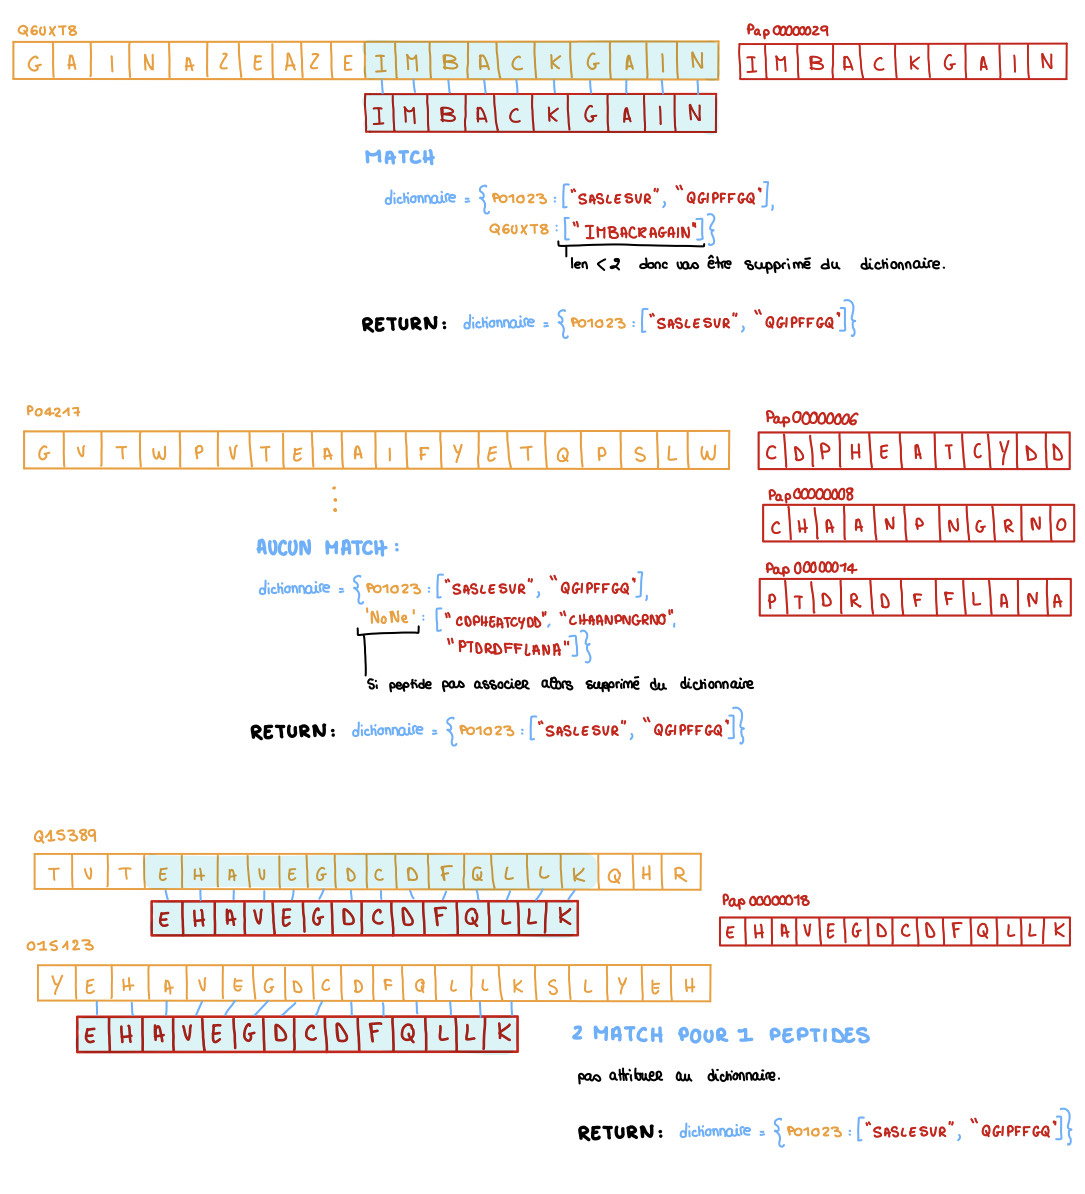
\includegraphics[width=6.5cm]{assemb_2.jpg} }}%
    \qquad
    \subfloat[\centering Exemple de refus des séquences invalides ]{{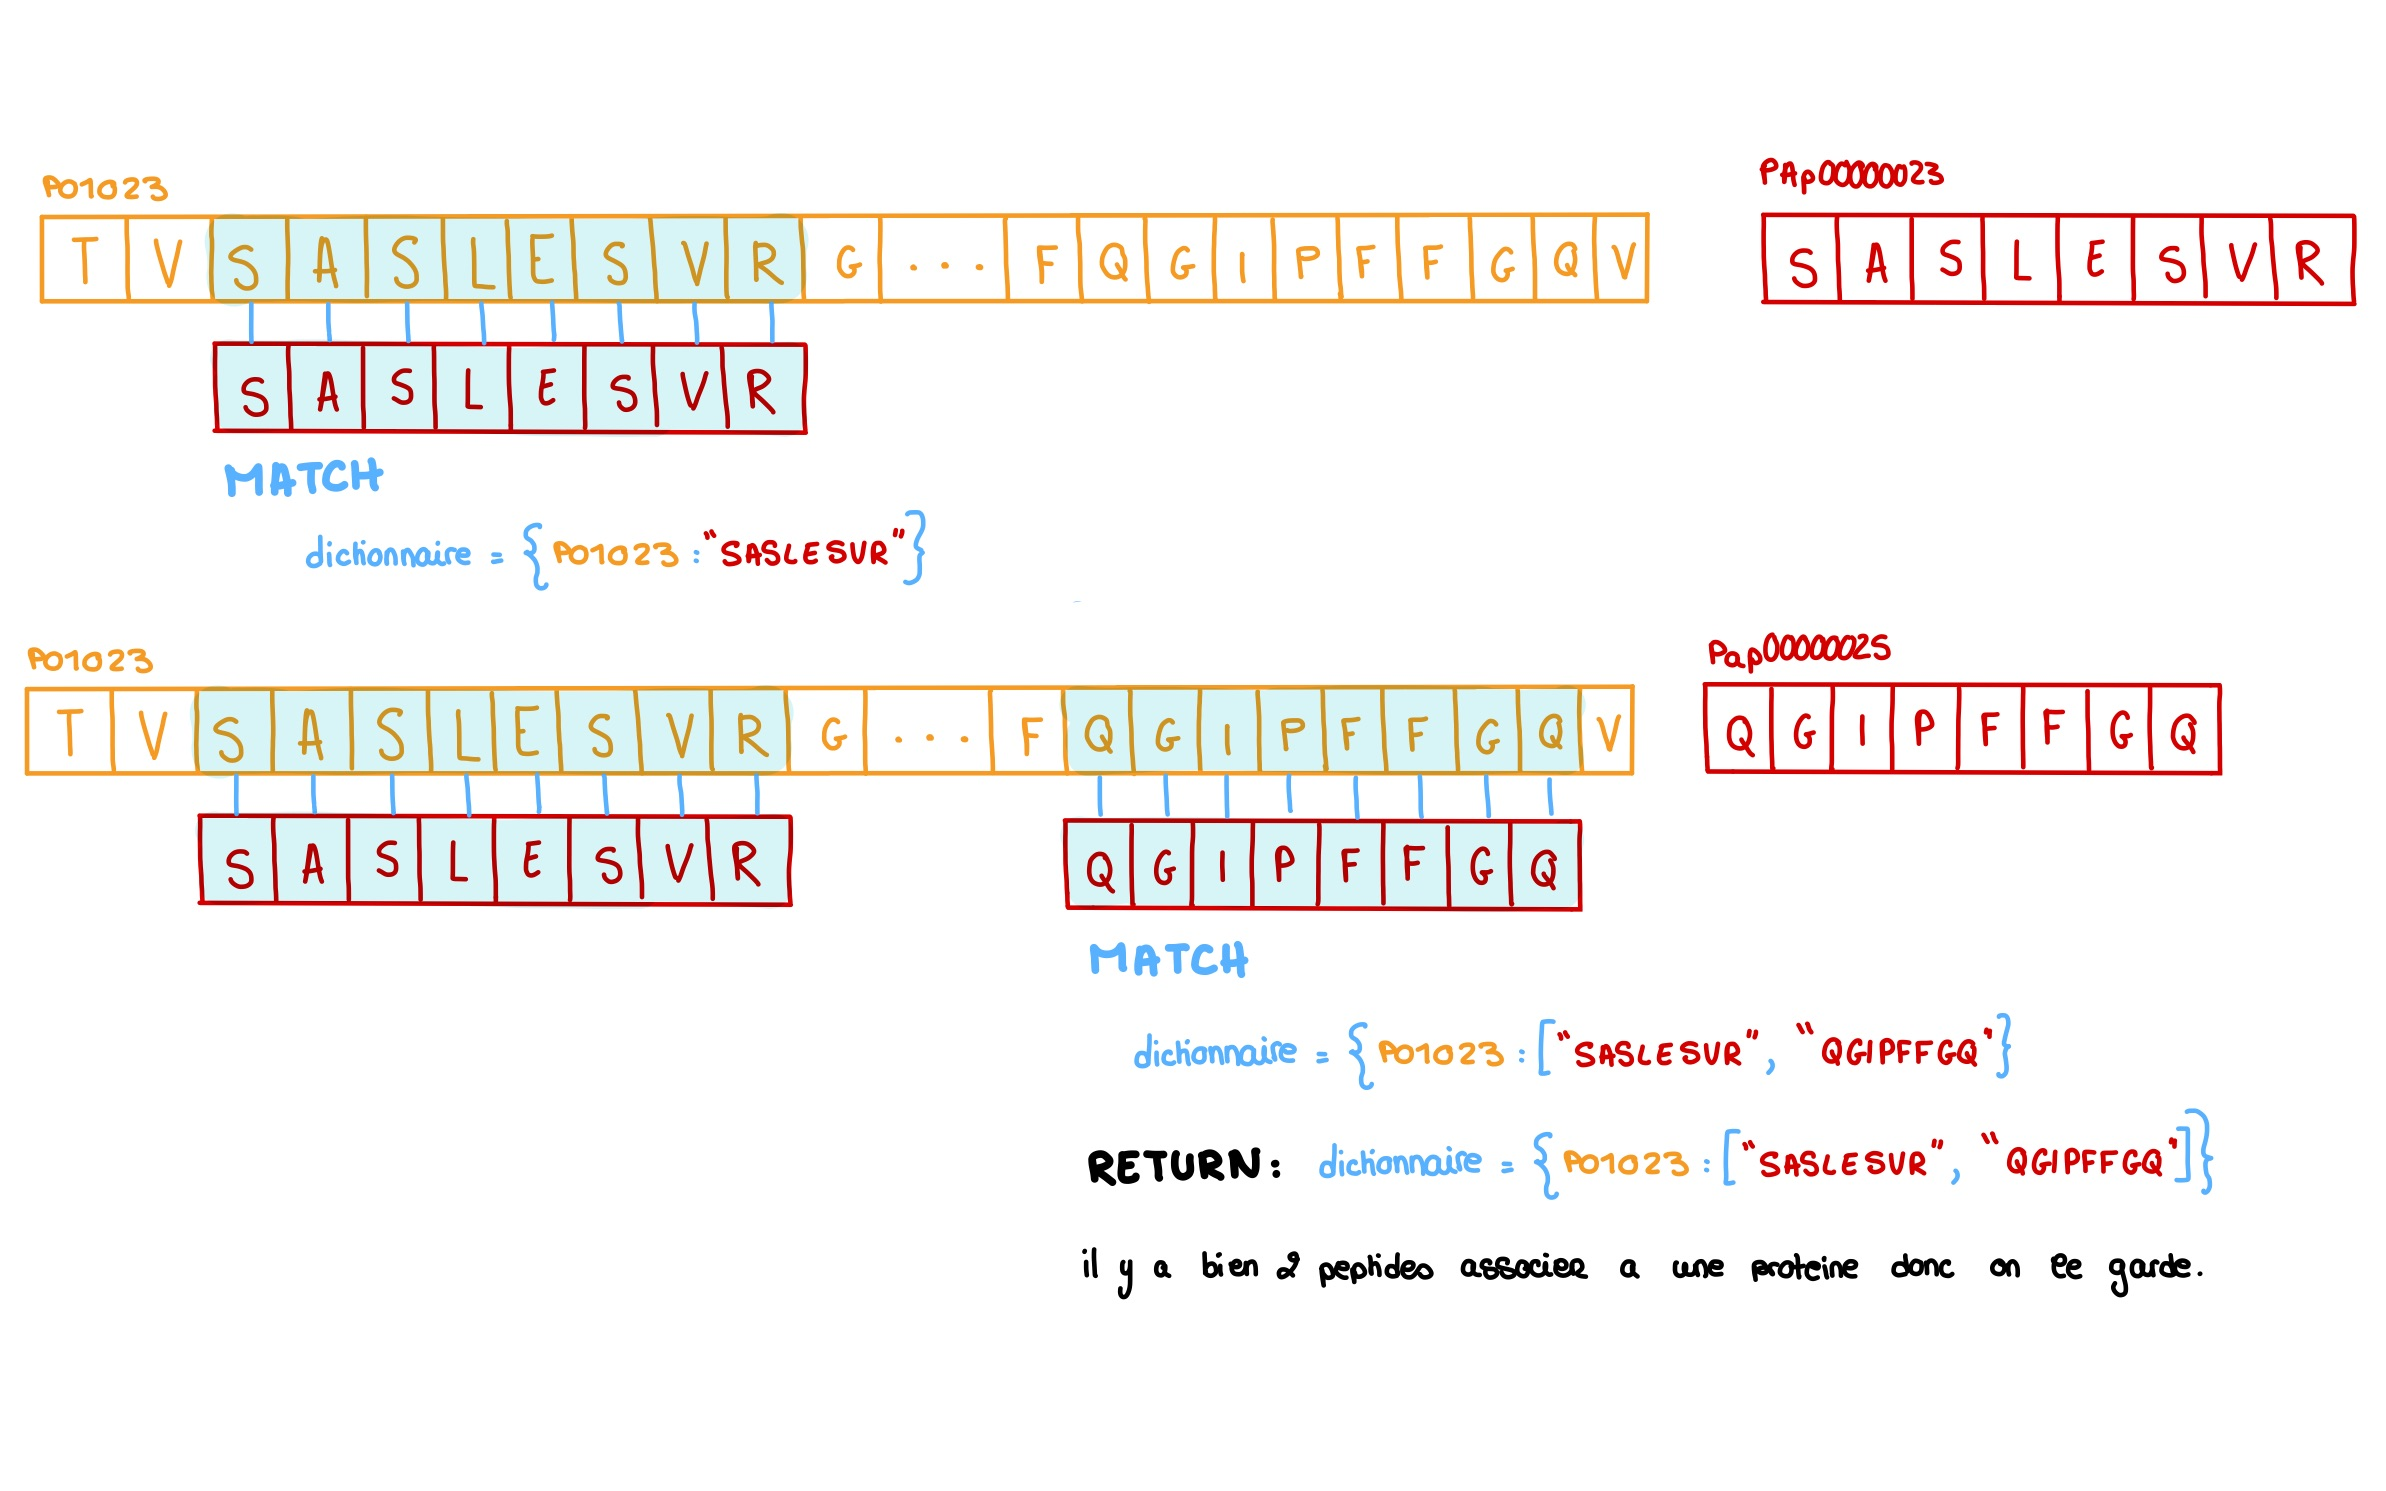
\includegraphics[width=7cm]{assemb_1.jpg} }}%
    \caption{Exemples d'exécution de la fonction unique\_match\_set sur des données réelles}
    \label{}%
\end{figure}


\begin{SCfigure}[][h]
\caption{Exemples d'exécution de la fonction assembely\_peptides sur des données fictives\vspace{1cm}}\label{}
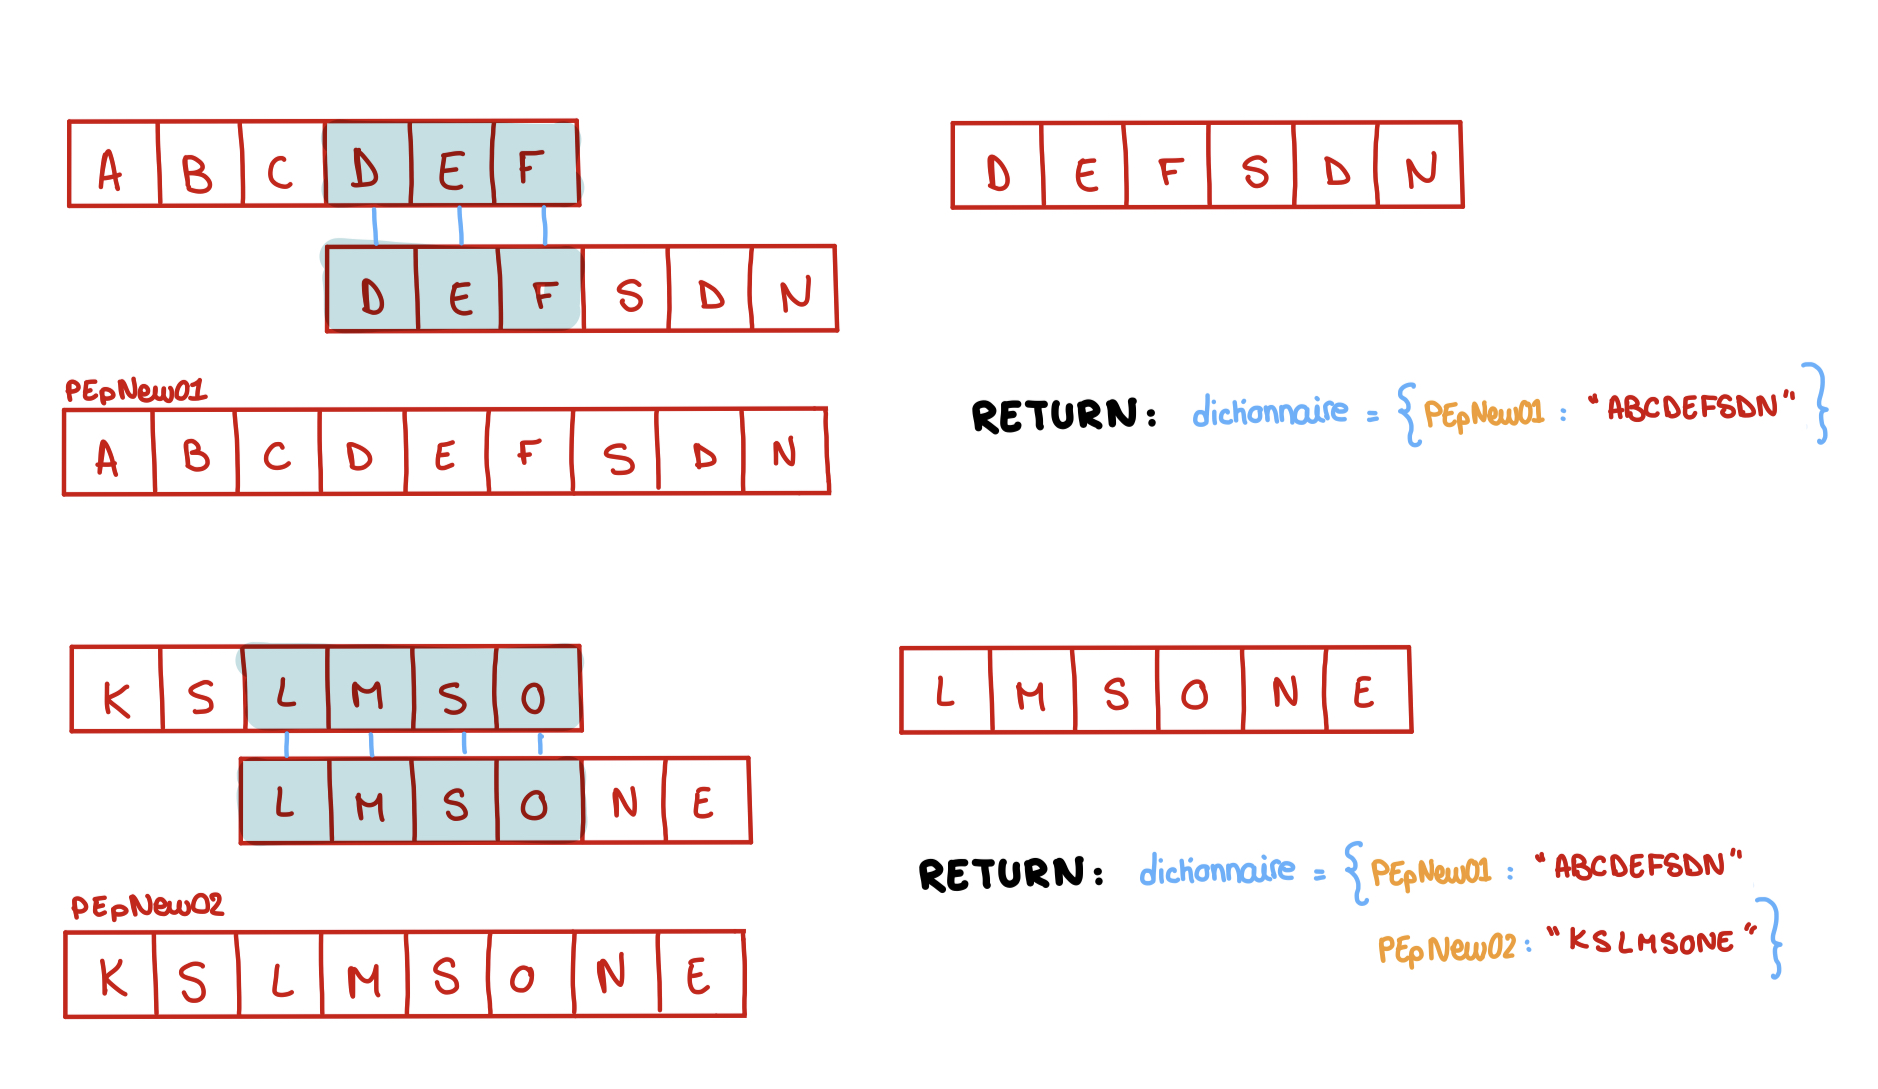
\includegraphics[width=0.3\textwidth]{overlap_sch.jpg}
\end{SCfigure}

\subsection{Similarité entre les mesures et le jeu de données}
\subsubsection{How close is your solution to the human\_blood protein set ?}
\hspace*{1cm} Notre banque de donnés contient un total de 772 protéines. En appliquant la fonction unique\_match\_set 365 d'entre elles possèdent au moins deux peptides uniques qui leurs sont associés. Cela représente 47,2 \% des protéines totales, ce qui pour des données biologiques semble être un très bon début.\\
\hspace*{1cm} Malheureusement, après avoir ajouté les peptides assemblés en sortie de la fonction assembely\_peptides, les 173 protéines identifiées faisaient toutes parties des protéines déjà reconnues. Il serait intéressant de refaire le pipeline en modifiant l'overlap min (ici a 15) pour obtenir plus de peptides d'assemblage. 

\subsection{Solution en cas concret}
\subsubsection{May your solutions be used on real world cases ?}
\hspace*{1cm} Afin de poser une base statistique sur nos affirmations, on réalise un test comparant la fraction des protéines identifiées au nombre total de protéines. 
\begin{quote}
    On observe que 47,2 \% des protéines du jeu de donné sont identifiées. 
    La proportion des protéines identifiées est significativement différente de la prorportion théorique (p < 0.0001 , X2 = 545, ddl = 1, test de comparaison de proportion à proportion, unilatéral). On conclut que l'échantillon étudié devrait être raffiné avant d'être utilisé en situation réelle.
\end{quote}

\subsection{Amélioration biologique}
\subsubsection{Can your identifier deal with all the biological cases ?}
\hspace*{1cm}La solution que nous avons produite semble prometteuse, en revanche, comme présentée dans la partie 2, la lenteur du script rend son utilisation en dur relativement complexe. Dans le cas où les mesures sont répètes et que l'analyse doit être menée plusieurs fois, le temps de calcul pourrait limiter les activités du laboratoire. \\
Malgré tout, les scripts produisent des résultats lisibles et ergonomiques, facilitant leur utilisation future. \\
\\
\hspace*{1cm} D'autre part, nos fonctions sont écrites de façon a limiter la plupart des erreurs liées aux défauts du jeu de données. En effet, chaque peptide doit être unique. De plus, un manque de précision dans les mesures sera comblé par la redondance de l'analyse, les protéines sont discriminées par au moins deux peptides et, le chevauchement minimal lors de l'assemblage de ces derniers permet d'assurer une bonne fiabilité des résultats.  


\section{Amélioration possible}
\subsection{Test de vitesse}
\hspace*{1cm}Notre fonction unique\_match\_set est relativement rapide, 12 minutes de calcul environ pour le jeu de donné entier. Par contre, la fonction assembly\_peptides est très chronophage. L'assemblage du fichier complet pour un overlap minimal à 15 a pris 8h40 en tout pour un total de 3410 peptides assemblés soit environ 7 peptides par minute. 
\begin{figure}[H]\centerline{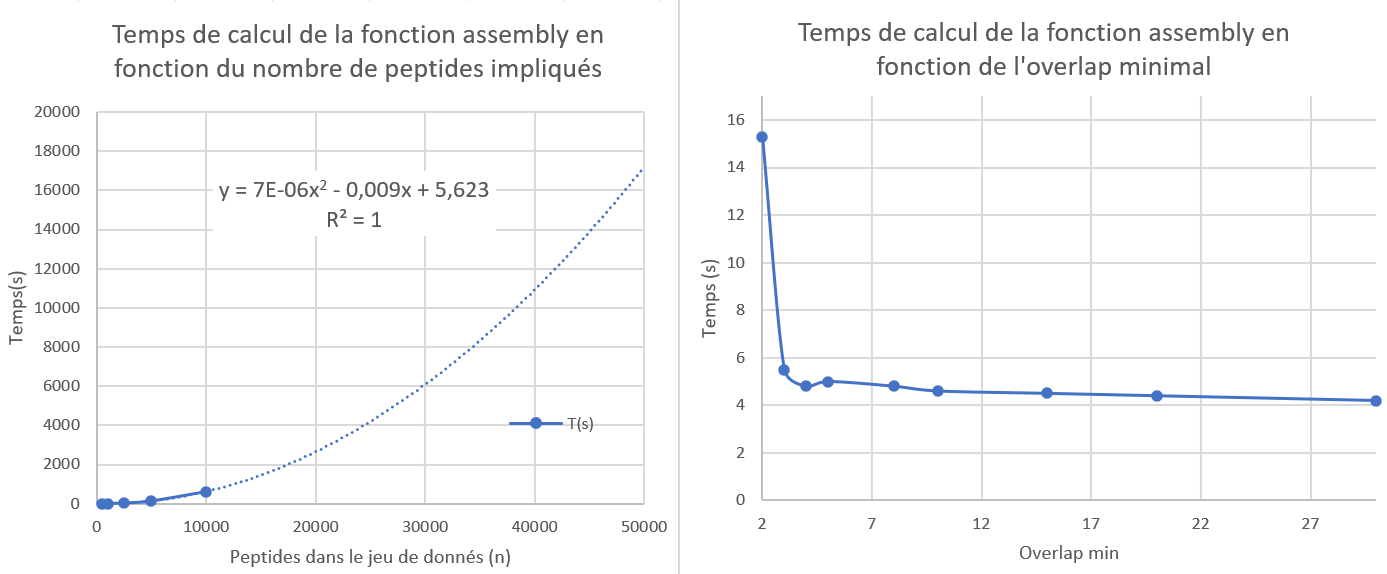
\includegraphics[width=1\textwidth]{overlap.png}}\captionsetup{justification=centering}
\caption{A gauche, temps de calcul de assembly\_peptides en fonction du nombre de peptides impliqués, la croissance du temps semble être polynomiale. A droite, le temps de calcul en fonction de l'overlap minimal, ce dernier ne semble pas avoir d'influence au-dessus de 2 }\end{figure}

\subsection{Perspectives d'amélioration}
\hspace*{1cm}Nos fonctions, ont déjà par le passé été codées et optimisées par de nombreux bioinformaticiens. En lisant les publications à ce sujet, on peut facilement identifier deux perspectives d'améliorations majeures pour notre code.
\begin{quote}
    Cock, P.\& de Hoon, M. (2009). Biopython: freely available Python tools for computational molecular biology and bioinformatic. in  Oxford University Press (OUP). https://doi.org/10.1093/bioinformatics/btp163
\end{quote}
\hspace*{1cm}Comme cité dans la publication sur le package "Biopython" le language C offre de bien meilleures performances pour les traitements répétitifs que nous faisons ici. De plus, l'ajout de "Multithreading" dans nos programmes, nous permettrait d'utiliser la puissance de nos machines à leurs pleins potentiels divisant le temps de calcul par le nombre de coeurs de notre CPU.\\ 
\begin{center}
   \href{https://github.com/SaraSpieler/OBI}{Touts les scripts et fichiers sont sur GitHub}
   \qrcode[height=1cm]{https://github.com/SaraSpieler/OBI}
\end{center}


\end{document}
